\chapter{Mitigazioni}

Nel capitolo precedente sono stati analizzati i principali azzardi individuati nell'apparato IMR e molti di questi sono stati classificati come \textit{intollerabili}; per questi ultimi � opportuno realizzare una procedura di mitigazione. La mitigazione pu� avere come scopo quello di ridurre la severit� dell'azzardo oppure renderlo meno frequente, in modo tale che possa venir considerato \textit{tollerabile} per il sistema. In questo capitolo+ sono descritte le due mitigazioni applicate all'apparato successivamente all'hazard analysis: 
\begin{itemize}
	\item utilizzo di una One Time Password;
	\item utilizzo del protocollo PVS.
\end{itemize}
Tramite l'utilizzo di una OTP infatti � possibile rendere tollerabili tutte le criticit� riscontrate nella fase di "Esecuzione comando AM" descritta nel capitolo precedente. Invece, attraverso l'utilizzo del protocollo PVS sono stati mitigati tutti i rimanenti azzardi.

\section{Utilizzo di una One Time Password}
Dall'analisi � risultato che la maggior parte della situazioni indesiderabili si verificherebbe quando l'AM tenta di eseguire un comando critico. Infatti � possibile che, a causa di un attacco esterno oppure accidentalmente, il messaggio contenente il comando venga eliminato o alterato, cos� come la risposta di conferma di esecuzione del comando. Per ovviare a tale problematica � stato pensato di aggiungere all'architettura dell'apparato un ulteriore dispositivo: lo Smartphone.\\
Tale dispositivo viene impiegato dal sistema quando l'AM ha intenzione di eseguire un comando critico per la sicurezza, con lo scopo di utilizzare un canale alternativo per convalidare il comando.\\ In particolare, quando l'AM decide di effettuare un comando critico, l'IMRS invia la richiesta di conferma del comando al Tablet; per attuare tale operazione, l'AM deve inserire sul Tablet una One Time Password pervenuta intanto sullo Smartphone tramite un canale alternativo. Quindi, una volta che l'IMRS riceve la richiesta di esecuzione di un comando critico, risponde:
\begin{itemize}
	\item al Tablet, inviando una immagine contenente il comando ricevuto, incluse alcune informazioni associate;
	\item allo Smartphone, inviando una informazione contenente il comando ricevuto e una OTP.
\end{itemize}
\begin{figure}[ht]
	\centering
	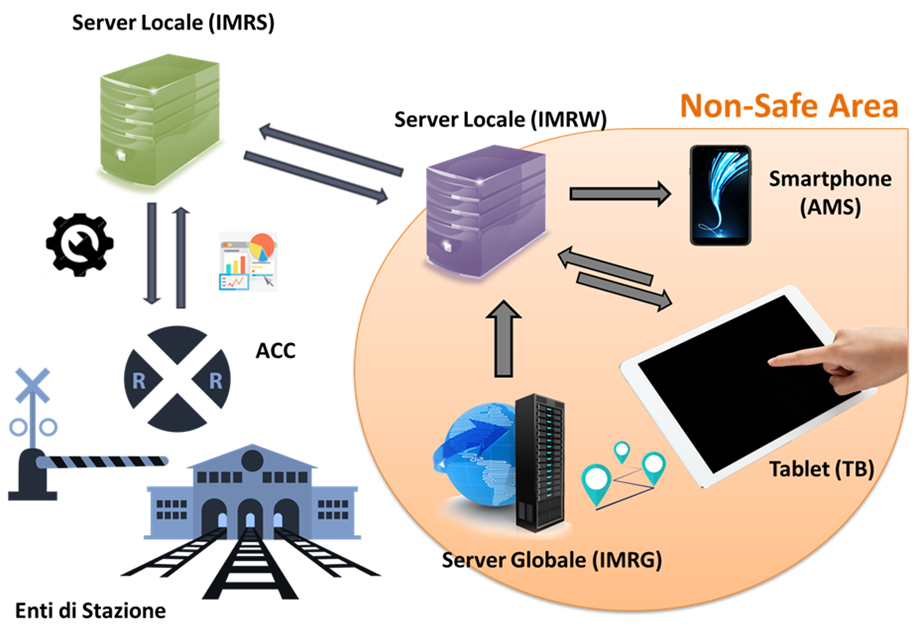
\includegraphics[width=0.8\linewidth]{img/architdue}
	\caption{Il ruolo dello Smartphone nell'apparato IMR}
\end{figure}
In questo modo l'AM pu� verificare la consistenza delle informazioni giunte su Tablet e Smartphone e in seguito inserire la OTP sul Tablet per confermare il comando. A questo punto il server IMRS potr� inoltrare il comando al nucleo in sicurezza, se la password risulta verificata.\\ Se il nucleo esegue il comando, viene inviata dal server IMRS:
\begin{itemize}
	\item al Tablet: una immagine che contiene la conferma del comando (o le informazioni richieste) e una nuova OTP;
	\item allo Smartphone: la stessa OTP e le informazioni accessorie per confermare i dati contenuti nell'immagine.
\end{itemize}
Attraverso questa procedura � possibile contrastare eventuali contraffazioni alle informazioni eseguite da un attaccante.\\
Invece, se il nucleo non esegue il comando, viene inviata una notifica solo verso il Tablet, senza OTP. Non avendo OTP da inserire, l'AM ne conclude che il comando non � stato eseguito.\\
Durante tutta la procedura appena descritta l'AM � direttamente responsabile di confrontare visivamente che le informazioni giunte sui dispositivi combacino, incluse le OTP. L'AM inoltre � anche responsabile di non assumere la corretta esecuzione del comando, qualora la procedura realizzata non rispetti lo schema descritto.\\ Nell'immagine seguente � possibile osservare il sequence diagram della fase \textit{Esecuzione comando} con gli aggiornamenti riguardanti l'aggiunta dell'utilizzo della OTP.
\begin{figure}[ht]
	\centering
	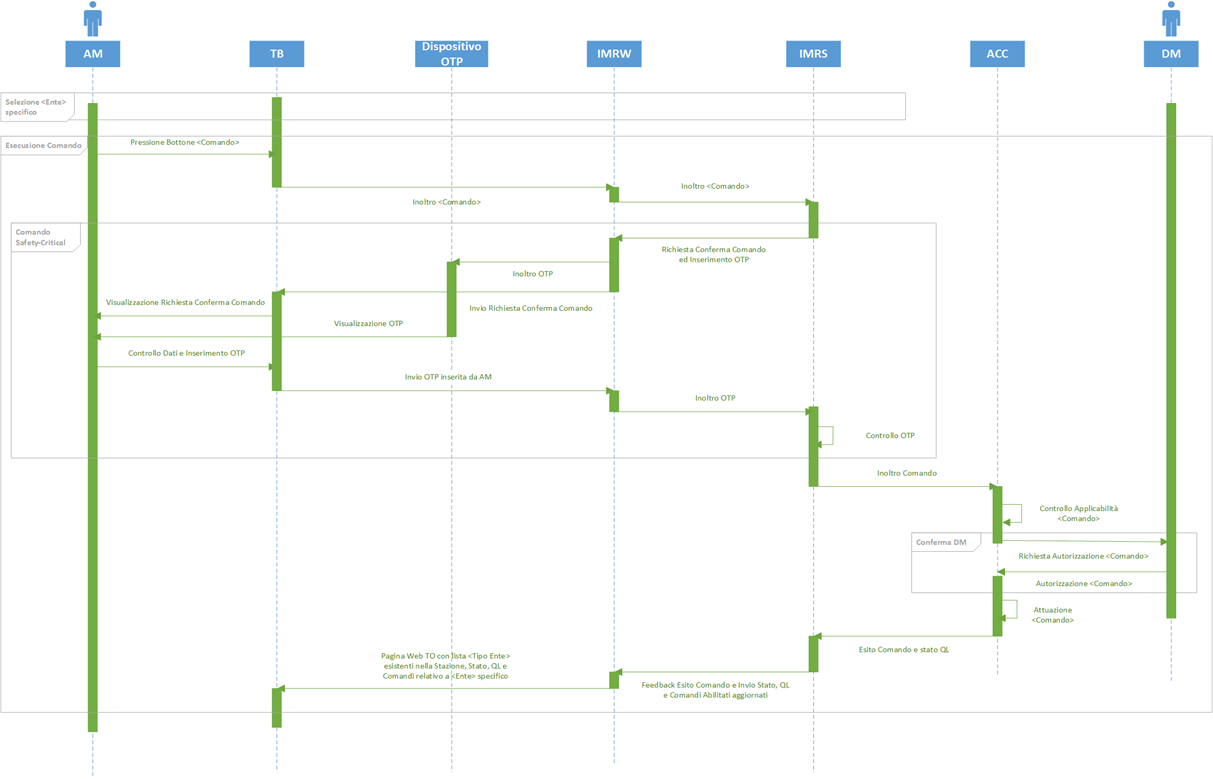
\includegraphics[width=1.1\linewidth]{img/sdesecuzione}
	\caption{Sequence diagram Esecuzione comando}
\end{figure}


\section{Utilizzo del protocollo PVS}
Poich� i canali di comunicazione ordinari non sono affidabili, l'apparato IMR adotta un protocollo noto come Protocollo Vitale Standard (PVS), ideato da RFI per consentire interazioni sicure tra diversi dispositivi. Per imporre la safety di tutte le comunicazioni la procedura deve essere progettata secondo lo standard EN50159 \cite{dodici} e dovrebbe essere codificata come linguaggio di medio-basso livello in accordo allo standard EN50128 \cite{undici}.\\ Il protocollo PVS fornisce un livello di safety insieme alla protezione contro l'accesso non autorizzato attraverso l'uso di codici di sicurezza e tecniche crittografiche. Le tecniche e gli algoritmi inclusi nel protocollo sono stati identificati tra quelli collaudati, validati e proven-in-use nel settore ferroviario.
\newline
Il protocollo pu� essere riassunto come un software aggiuntivo che fornisce le funzionalit� OSI di sessione e presentazione tramite:
\begin{itemize}
	\item codici di sicurezza (per garantire l'integrit� del messaggio);
	\item numero di sequenza (per evitare la re-sequenziazione, ripetizione, inserimento e cancellazione di messaggi);
	\item execution cycle (per ottenere la freshness del messaggio);
	\item identificativi di nodo, sorgente e destinazione, univoci (per l'autenticit�);
	\item crittografia.
\end{itemize}
Dall'unione di questi meccanismi � possibile garantire comunicazioni sicure.
\newline
La comunicazione bidirezionale tra IMRS e IMRW � condotta tramite messaggi scambiati attraverso il protocollo PVS, di conseguenza entrambi i server dovranno aprire un canale di comunicazione bidirezionale.\\
Invece l'interazione tra il server IMRW e il Tablet prevede una procedura pi� articolata:
\begin{itemize}
	
 \item il server genera delle pagine HTML tramite opportuno linguaggio di scripting lato-server;
 \item questo flusso HTTP viene intercettato da uno script, il PVS Server, che prende il messaggio e lo usa come payload per una comunicazione PVS;
 \item il messaggio PVS cos� creato viene inviato al Tablet su una porta predefinita sulla quale ascolta il modulo PVS Client;
 \item il modulo PVS Client, dopo aver ricevuto i dati PVS, li decapsula e li reinoltra sulla porta HTTP (default: 80) del Tablet. 
\end{itemize}
 Quando l'AM vuole inviare dei comandi tramite TB al server IMRW, verr� eseguito il procedimento a ritroso, sfruttando lo stesso canale sicuro.
 \begin{figure}[ht]
 	\centering
 	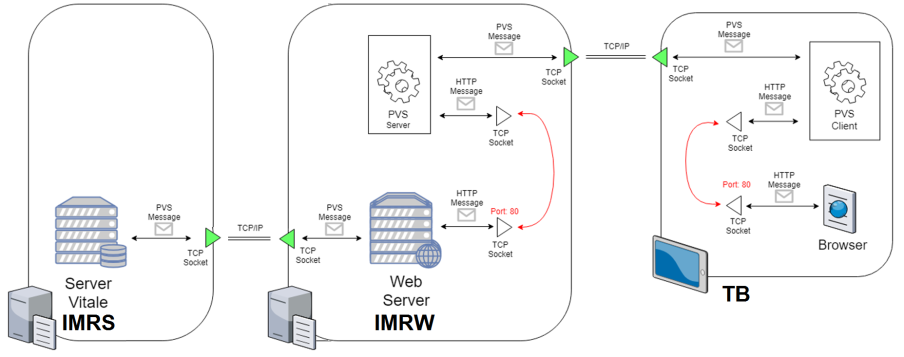
\includegraphics[width=0.9\linewidth]{img/pvs}
 	\caption{Protocollo PVS}
 \end{figure}
 

\section{Direttive comportamentali}
Tramite l'utilizzo delle due mitigazioni appena descritte, tutti i rischi classificati come \textit{intollerabili} nel capitolo precedente, possono venir rivalutati e considerati invece come \textit{ammissibili} per l'apparato IMR. Infatti, attraverso l'uso del protocollo PVS e della procedura che prevede l'inserimento delle OTP, la safety del sistema non � pi� a rischio. \\
Di seguito sono state inserite alcune linee guida per l'utilizzo del sistema, per cercare di ottimizzare l'impiego di quest'ultimo:
\begin{itemize}
	\item \textit{avere a disposizione un tablet di riserva}: questo accorgimento � necessario quando il tablet utilizzato dall'operatore non riesce a eseguire correttamente le operazioni di base (touchscreen non reattivo, spegnimento improvviso del tablet, mancata gestione della batteria ecc..);
	
	\item \textit{riaggiornamento pagina}: da effettuare quando ad esempio la lista delle stazioni non � completa;
	
	\item \textit{utilizzare password potenti}: per fare in modo che il meccanismo di autenticazione tramite password sia solido e sia difficile per un attaccante introdursi nel sistema � necessario che la password adottata sia pi� complessa possibile. E' quindi consigliabile utilizzare sia lettere maiuscole che minuscole, segni e numeri;
	
	\item \textit{numero tentativi autenticazione limitati}: � possibile che un attaccante per accedere al sistema abbia intenzione di provare tutte le password di un dizionario. Per evitare che tale attacco sia possibile, � necessario imporre che i tentativi di autenticazione siano limitati, ad esempio un numero appropriato di tentativi di autenticazione potrebbe essere pari a 3;
	
	\item \textit{modificare la password periodicamente}: per garantire la sicurezza del sistema � opportuno che le password degli addetti manutenzione vengano modificate periodicamente;
	
	\item \textit{memorizzare la chiave privata in sicurezza}: per evitare che il file contente la chiave privata possa essere reperibile da individui non autorizzati ad accedere al sistema, � opportuno che venga salvato in una posizione di massima sicurezza;

	\item \textit{effettuare l'autenticazione periodicamente}: per fare in modo che il Tablet non possa essere utilizzato da terzi per l'esecuzione di comandi, sarebbe bene che periodicamente venga effettuata l'operazione di login da parte dell'AM.


\end{itemize}